\documentclass[journal]{IEEEtran}

\usepackage[nomain, acronym, symbols]{glossaries}
\usepackage[english]{babel}
\usepackage[hidelinks]{hyperref}
\usepackage{doi}
\usepackage{multirow}
\usepackage[table,xcdraw]{xcolor}
\usepackage[numbers]{natbib}
\usepackage{algorithm}
\usepackage{algorithmic}
\usepackage{graphicx}
\usepackage{amsmath,amsfonts,amssymb}
\usepackage{amsthm}
\usepackage{mathtools}
\usepackage{tikz}
\usepackage{placeins}
\usepackage{float}
\usepackage[caption=false]{subfig}
\usepackage{tikz}
\usepackage{microtype}

\usetikzlibrary{positioning, arrows.meta, fit, backgrounds, shapes.geometric}

\loadglsentries{acronyms}

\begin{document}

\title{Adaptation and Evaluation of an Energy-Aware, Multicore, Real-Time Scheduler on RISC-V}

\author{
    \IEEEauthorblockN{Eric Fernandes Evaristo, José Luis Conradi Hoffmann, Antônio Augusto Fröhlich} \\
    \IEEEauthorblockA{
        \textit{Software/Hardware Integration Lab (LISHA), Federal University of Santa Catarina (UFSC) Florianópolis, Brazil} \\
        \{fernandes, hoffmann, guto\}@lisha.ufsc.br
    }
}

\maketitle

\IEEEpeerreviewmaketitle

\begin{abstract}
    The portability of \gls{ml}-driven \gls{dvfs} frameworks across fundamentally different micro-architectures remains largely unexplored. This research investigates the portability of an online \gls{ml}-based energy-aware scheduler, originally built for ARM, by adapting it to a multicore RISC-V platform. Using performance counter-driven \glspl{ann}, the framework predicts \gls{dvfs} impacts to minimize energy consumption without violating hard real-time constraints. To adapt to RISC-V, the original feature selection pipeline was modified to filter idle noise and avoid task-specific features. Evaluations demonstrate the framework successfully adapts to dynamic workloads, reducing energy consumption by up to 58.54\% with minimal runtime overhead. However, cross-architectural comparisons reveal that the predictive model does not fully transfer to different platforms without adaptations, and observed hardware metric limitations occasionally induced incorrect task migrations.
\end{abstract}

\begin{IEEEkeywords}
RTOS, Energy Optimization, Machine Learning, Scheduling, RISC-V
\end{IEEEkeywords}

\section{Introduction}

Real-time embedded systems are subject to strict power budgets, driven by constraints such as battery capacity and thermal dissipation limits \cite{rahim2025survey}. Among the sources of power consumption in these systems, dynamic power is particularly relevant because it scales with the square of the supply voltage and linearly with the operating frequency. \acrfull{dvfs} exploits this relationship, allowing the processor to trade off computational throughput for lower power consumption \cite{ul2018task}. However, frequency directly determines how fast instructions are executed and, consequently, how long a task takes to execute. In periodic real-time task sets, each task is associated with a deadline that must be met. When overall CPU utilization leaves sufficient slack time, the processor can operate at a lower frequency while still meeting all deadlines \cite{ul2018task}. Reducing the operating frequency whenever there is sufficient scheduling slack is therefore a practical strategy for improving energy efficiency \cite{hoffmann2021online}.

The key challenge is identifying how much we can reduce the frequency without causing any task to miss its deadline \cite{ul2018task, hoffmann2021online}. This is not trivial in modern multicore systems, where tasks share not only processor cores but also memory buses, caches, and hardware accelerators. Unlike single-core platforms, where timing behavior can be soundly characterized in isolation, a task running on a multicore system cannot be treated independently: inter-core contention for shared resources can substantially inflate execution times depending on which tasks are co-scheduled, and exhaustively covering all possible allocation combinations through offline testing quickly becomes intractable as the number of tasks and cores grows. Furthermore, offline testing cannot account for the dynamic workloads of modern systems, where tasks may be created, suspended, or destroyed at runtime \cite{gracioli2019designing, horstmann2019framework, lugo2022survey}. Hardware performance counters provide a direct view into these architectural effects at runtime \cite{hoffmann2021online}. By selecting the most informative counters about resource contention and combining them with carefully tailored \acrfull{ml} algorithms, it is possible to capture the timing behavior of individual tasks under varying conditions, without requiring offline worst-case analysis for every possible co-runner combination and without imposing significant overhead on task execution \cite{hoffmann2021online}.

\gls{ml} has gained increasing relevance in real-time scheduling in recent years \cite{rahim2025survey, ul2018task}. Hardware performance counters have also shown to be effective at capturing micro-architectural behavior at runtime \cite{mazzola2022data}, making them useful inputs for such models \cite{hoffmann2021online}. Applying these concepts, our prior work \cite{hoffmann2021online} proposed an \gls{oleamrts}, demonstrating that the usage of performance counters enables accurate prediction of task utilization in real-time multicore systems, an approach subsequently extended and validated on an ARMv8 platform \cite{hoffmann2024lightweight}. In this paper, we build upon that methodology and adapt the \gls{oleamrts} to a RISC-V platform to assess how well the approach generalizes across architectures and identify the conditions under which it fails to achieve satisfactory results.

The main contributions of this paper are the following:
\begin{itemize}
    \item A validation of an adapted \gls{ml}-guided, energy-aware scheduler across multiple architectures with distinct hardware characteristics, extending the original implementation and analysis;
    \item An adapted feature selection pipeline for RISC-V.
    \item An empirical overhead analysis of the scheduler in a hard real-time context for a new platform with RISC-V architecture.
\end{itemize}

\section{Related Works}

The present work builds directly on two prior publications from our research group. Hoffmann and Fröhlich \cite{hoffmann2021online} introduced \gls{oleamrts}, an \acrfull{ann}-based runtime energy optimizer that uses hardware performance counters and \gls{os} statistics to predict the impact of frequency scaling on task performance in a multicore real-time system. The predictor is trained online whenever \gls{dvfs} is applied, allowing it to adapt to the running task-set without requiring offline profiling for each possible configuration. This was subsequently extended in \cite{hoffmann2024lightweight}, where a locking problem was identified: when the ANN warm-start leads to overestimated utilization predictions, \gls{dvfs} actuation is blocked and online learning cannot proceed. An unlocking procedure was proposed and validated on ARMv8, but the framework had not yet been evaluated on architectures with fundamentally different \gls{pmu} designs or more aggressive \gls{dvfs} granularity. The present work addresses this gap by porting and validating \gls{oleamrts} on a RISC-V platform.

Despite the growing relevance of \gls{ml}-based approaches to energy optimization in real-time multicore systems, recent works rarely exploit \gls{pmu} counters as a primary source of runtime information \cite{rahim2025survey}. Energy-aware schedulers frequently employ \gls{rl} driven by coarse system metrics such as overall CPU utilization \cite{li2025energy, uddin2023dynamic}, which, besides introducing higher computational costs, fail to capture the shared resource contention that dictates execution delays in multicore environments. On the hardware monitoring side, however, Mazzola et al. \cite{mazzola2022data} demonstrate that performance counters can effectively capture this complex architectural behavior through a systematic feature selection pipeline, achieving an accurate, platform-agnostic power estimation model. More broadly, \gls{ml}-driven schedulers remain affected by poor generalization across platforms and workloads. While online learning is acknowledged as a way to mitigate this, developing a cross-platform, portable, and real-time capable solution remains a major challenge, further complicated by inference and training overhead and scalability concerns for larger task and core counts. Our framework builds upon these concepts, combining \gls{pmu}-driven hardware-informed inputs with continual online learning, and is here adapted and evaluated on a new architecture to assess how well this approach generalizes in practice.

\section{System Model} \label{sec:system_model}

To evaluate the portability of \gls{oleamrts}, we adopt a standard multicore real-time scheduling model \cite{ul2018task}, augmented with the specific micro-architectural constraints imposed by the target \gls{cots} RISC-V platform.

We consider a multicore \gls{soc} comprising a set of identical hardware threads (harts), denoted as $M = \{m_1, m_2, \dots, m_W\}$. The system supports \gls{dvfs}, providing a finite set of discrete operating frequencies ${F = \{f_{min}, \dots, f_{max}\}}$. Dynamic power dissipation scales proportionally to the voltage and frequency ($P \propto V^2f$). Crucially, the cores in $M$ are not necessarily independently scalable. They are organized into frequency clusters (or voltage/frequency domains). Let $V = \{v_1, \dots, v_K\}$ be the set of clusters, where each cluster $v_k \subseteq M$ shares a single clock and voltage supply. Consequently, a \gls{dvfs} actuation applied to any core $m \in v_k$ simultaneously forces all cores within $v_k$ to transition to the newly selected frequency $f \in F$.

The workload consists of a task-set $\Gamma = \{\tau_1, \tau_2, \dots, \tau_N\}$ of independent, periodic, or sporadic real-time tasks. At the operating system level, tasks are scheduled using \gls{pedf}. The global task-set $\Gamma$ is statically partitioned into disjoint subsets $\Gamma_m$ assigned to each core $m \in M$. Each task $\tau_i$ is formally defined by the tuple $(C_i, D_i, P_i)$, representing its \gls{wcet} measured in strict isolation at maximum frequency, its relative deadline, and its period, respectively.

We assume constrained or implicit deadlines ($D_i \le P_i$). Under dynamic runtime conditions, the actual execution time of a job belonging to task $\tau_i$, denoted as $C_{i_{actual}}$, might deviate significantly from $C_i$. This deviation is a nonlinear function of the assigned cluster frequency $f \in F$ and the inter-core interference $I(t)$ generated by co-scheduled tasks contending for shared resources (e.g., memory buses and shared cache). This non-linearity occurs because CPU-bound operations scale directly with frequency, whereas memory and I/O latency are frequency-independent but susceptible to multicore interference. Because a frequency downscale affects all cores in $v_k$, the objective of the framework is to predict $C_{i_{actual}}$ under lower frequencies to actuate \gls{dvfs} safely at the cluster level, ensuring $C_{i_{actual}} \le D_i$ for all tasks in $v_k$ while minimizing energy consumption.

Lastly, the model accounts for a \gls{pmu}, which tracks a set of available architectural events ${E = \{e_1, e_2, \dots, e_X\}}$ using a finite set of hardware counters $H = \{h_1, h_2, \dots, h_Y\}$. These events provide the runtime metrics necessary to quantify shared resource contention. To track these counters without introducing significant overhead or interference, we assume a non-intrusive monitoring architecture, such as the framework proposed by Horstmann et al. \cite{passig2023monitoring}.

\section{Architecture-Agnostic Predictive Framework}

To maximize energy savings via \gls{dvfs} without violating real-time constraints, the scheduler must accurately predict execution delays caused by shared resource contention. To achieve this, the framework employs a lightweight, feed-forward \gls{ann} and a core migration heuristic. To ensure the non-intrusiveness of the solution, all framework operations, except for task data monitoring, are executed on a dedicated system core. Prediction and migration routines also only actuate at the boundaries of every hyper-period, which is the time required for the entire system behavior to repeat. This is formally defined as the least common multiple of all task periods, i.e. $HP = \text{lcm}(P_1, P_2, \dots, P_N)$. Tasks are evaluated using a job-based monitoring mechanism. Whenever a job finishes, it registers a data vector containing its actual execution time, the current cluster frequency, and the growth rate of all relevant \gls{pmu} counters. These vectors are accumulated for each task across the hyper-period and then fed into a sliding window dataset restricted to the $n$ most recent entries, where $n$ is arbitrarily defined based on the temporal relevance of the data and performance constraints. Each entry is subsequently normalized: execution time is normalized against the hyper-period length, yielding the task utilization for that window, while the remaining hardware metrics are scaled using min-max normalization. Min-max was maintained from the original work for its low impact on performance.

The framework relies on an initial architectural profiling process utilizing a task-set designed to stimulate shared resource contention (detailed in Section \ref{sec:task-sets}). Data collected during this profiling phase establishes a system warm-start, providing the baseline model with the necessary inputs to predict execution times across different frequency levels. Furthermore, to avoid relying on vendor-specific heuristics, this profiling data is fed into a feature selection pipeline that identifies the specific \gls{pmu} events that capture these micro-architectural bottlenecks through statistical analysis of profiled data from the \gls{rtos} execution.

The framework maintains one dedicated \gls{ann} instance per core. Each \gls{ann} predicts the utilization of all locally assigned tasks for the upcoming hyper-period, simulating a hypothetical transition to the next lowest \gls{dvfs} level. These task-level predictions are then aggregated by core. If the total predicted utilization for every core remains strictly below $1 - SM$, where $SM$ is a predefined safety margin, the cluster frequency is safely scaled down. Note that $SM$ can be adjusted according to the variance in the performance traces of tasks. The \glspl{ann} continually adapt to dynamic workloads through online learning using the runtime collected data. Whenever the frequency is scaled down, the framework calculates the prediction error of the \glspl{ann}. If this error exceeds a predetermined tolerance, an incremental retraining phase is triggered, during which a limited number of training iterations are performed to bound the computational overhead.

The framework also features a migration heuristic for load balancing, with the objective of finding the optimal task allocation for frequency reduction. The heuristic utilizes the variance in \gls{pmu} counter growth rates to distribute tasks in a way that reduces contention, applying a \gls{mst} to inhibit low-benefit migrations. In the baseline framework, if a counterproductive migration occurs (e.g., one that prevents \gls{dvfs} actuation at the highest level), it is immediately revoked, and the \gls{mst} is increased. In this work, the heuristic is adapted to apply a secondary, lighter \gls{mst} increase whenever a migration fails to yield a lower frequency level. This prevents the tasks from being migrated indefinitely when the task-set cannot sustain further \gls{dvfs} downscaling.

\subsection{Profiling and Feature Selection}

Because the \gls{pmu} can only track a limited number of events simultaneously, offline data collection requires multiple passes over the profiling task-set, each configured with a different subset of \gls{pmu} events. The resulting traces are merged and aligned by timestamps into a single complete dataset, a process only feasible in an \gls{rtos} with a low interference profile, such as \gls{epos}. Data collected during this profiling phase establishes a system warm-start.

During pre-processing, cumulative counter data is converted into growth rates. An idle-thread noise filter was also introduced: average counter growth rates recorded during system idle periods are subtracted from the active tasks' growth rates (clamped to zero) to prevent background system events from skewing the data. Task utilization is calculated as the proportion of execution time relative to the task period ($\frac{C_{i_{actual}}}{P_i}$), rather than the \gls{wcet} ($\frac{C_{i_{actual}}}{C_i}$), and counter values are mathematically scaled by this instantaneous utilization prior to min-max normalization, establishing a temporal weighting that highlights the absolute architectural impact of a task.

The feature selection pipeline was adapted from the baseline, as the original pipeline was yielding task-specific counters, such as \gls{jalr} instructions and conditional branches, rather than generalized contention indicators, producing features that failed to yield relevant predictive results. The adapted pipeline employs two stages. First, \gls{pcc} acts as a baseline filter to quantify the linear relationship between architectural events and execution delays. Any feature exhibiting a \gls{pcc} correlation greater than 85\% with an already selected feature is pruned to maximize informational value within strict \gls{pmu} channel limits. Second, \gls{lassocv} is applied as an embedded regression method to shrink highly collinear features to zero via L1 regularization. The absolute \gls{lassocv} coefficients ($\beta$) are min-max normalized ($\widehat{\beta}$) and combined with the \gls{pcc} values into a composite relevance score: $Score = 0.25 \cdot PCC + 0.75 \cdot \widehat{\beta}$. Notably, \gls{igr} was excluded, as its sensitivity to counter discretization caused it to erroneously prioritize highly task-specific events (e.g., integer divisions) over generalized indicators of architectural contention.

\section{Experimental Evaluation}

To empirically validate the architecture-agnostic capabilities of the proposed predictive framework, all evaluations were conducted on a modern \gls{cots} RISC-V development platform: the StarFive VisionFive 2 \gls{sbc}. Powered by the JH7110 \gls{soc}, this platform features a quad-core SiFive U74 (RV64GC) 64-bit processor cluster. The memory hierarchy includes 32KB private L1 instruction and data caches per core, backed by a unified, shared 2MB L2 cache. The platform supports \gls{dvfs} at the cluster level, providing four discrete operating frequencies ranging from 375 MHz to 1.5 GHz. For hardware monitoring, the \gls{pmu} offers 27 core-local events (trackable via 2 fixed and 2 programmable counters) and 20 global L2 cache events (trackable via 6 programmable counters).

\textbf{Real-Time Operating System:} To guarantee deterministic execution and precisely measure micro-architectural overheads without the scheduling noise inherent to general-purpose operating systems, the framework was implemented within \gls{epos} \cite{epos}. \gls{epos} is a component-based \gls{rtos} designed to deliver strict timing guarantees for cyber-physical applications. The \gls{ann} and the contention-aware migration heuristic were integrated directly into the \gls{epos} kernel. Specifically, these routines are embedded within the real-time scheduler and execute during the idle periods of the dedicated framework core \cite{horstmann2019framework}. To interface with the RISC-V hardware, \gls{epos} accesses the local \gls{pmu} counters directly via system registers, while global L2 counters are accessed through \gls{dma} mappings within the L2 cache controller's memory region.

\textbf{Workload Configuration and Scaling:} To evaluate the framework, we adopt three tasks from the baseline methodology \cite{hoffmann2021online}, designed to trigger shared resource contention across distinct execution behaviors, and scale their computational demands to exceed the architectural limits of the JH7110 \gls{soc}. The CPU-Hungry task is a purely CPU-bound iterative Fibonacci generator that sustains deep pipeline saturation via floating-point arithmetic. The Bandwidth task is a memory-bound application that performs array traversals scaled to a 2MB \gls{wss}, severely oversubscribing the shared L2 cache and inducing continuous pipeline stalls. Instances are designated as "light" if they fit within the L1 cache, or "heavy" if they stress the L2. Finally, the Image Disparity task is a hybrid workload computing the disparity between two grayscale matrices, with its input size doubled (to $181\times136$) to prevent L1 cache encapsulation, ensuring its non-linear memory access patterns generate the severe inter-core interference necessary to properly evaluate the framework.

\subsection{Task-Set Configurations} \label{sec:task-sets}

To evaluate the framework's adaptability to RISC-V contention, we adapted the baseline task-sets, presented in the Table \ref{tab:task-sets}, doubling their periods to preserve original utilization proportions. Tasks execute on cores 1–3, reserving core 0 exclusively for \gls{oleamrts} operations. We designed three specific configurations to isolate offline profiling from continuous runtime adaptation. The first task-set (TS1, Homogeneous Warm-Start) features uniform periods to force persistent contention, serving as the offline workload to warm-start the \gls{ann}. The second (TS2, Heterogeneous Temporal Adaptation) introduces period variance, creating transient contention spikes that force the \gls{ann} to adapt entirely via online learning. Finally, the third task-set (TS3, Asymmetric Contention Stress) heavily oversubscribes Core 3 with diverse memory demands to explicitly trigger and validate the contention-aware migration heuristic, also relying purely on online adaptation.

\begin{table}[htb]
    \caption{Task-Set Configurations (BW-H/L: Bandwidth Heavy/Light, ID: Image Disparity, CPU: CPU-Hungry).}
    \label{tab:task-sets}
    \centering
    \footnotesize 
    \begin{tabular}{|c|c|l|}
        \hline
        \textbf{Set} & \textbf{Core} & \textbf{Assigned Tasks: Type (P/WCET in $\mathbf{ms}$)} \\ \hline
        \multirow{3}{*}{\textbf{TS1}}
         & 1 & BW-H (1000/200), ID (1000/200) \\
         & 2 & ID (1000/200), CPU (1000/200) \\
         & 3 & CPU (1000/200), ID (1000/200) \\ \hline
        \multirow{3}{*}{\textbf{TS2}}
         & 1 & BW-H (500/100), ID (1000/200) \\
         & 2 & ID (1000/400), CPU (500/70) \\
         & 3 & CPU (250/40), ID (500/200) \\ \hline
        \multirow{4}{*}{\textbf{TS3}}
         & 1 & BW-L (200/20) \\
         & 2 & BW-L (200/10), ID (2000/800) \\
         & 3 & CPU (200/60), ID (1000/200), \\ 
         &   & CPU (500/120), BW-L (2000/200) \\ \hline
    \end{tabular}
\end{table}

\subsection{Feature selection}

To perform comprehensive profiling and feature selection, 13 distinct executions of task-set 1 were required to aggregate data across all available hardware events. Performance traces were sampled periodically at a frequency of 34Hz in order to match the sampling rate of the original work. Based on the evaluation pipeline described previously, the final subset of selected architectural events is detailed in Table \ref{tab:selected_features}.

\begin{table}[htb]
    \caption{Selected Performance Counters and Relevance Scores}
    \label{tab:selected_features}
    \centering
    \footnotesize
    \begin{tabular}{|lcc|}
        \hline
        \textbf{Hardware Event} & \textbf{\gls{pcc}} & \textbf{\gls{lassocv} $\boldsymbol{\widehat{\beta}}$} \\ \hline
        L2 Acquire Block Hit & 0.04 & 1.00 \\
        L2 Release Data (Modified to Invalid) & 0.56 & 0.67 \\
        CPU Cycles & 0.45 & 0.21 \\
        Outer Acquire Block Miss (Invalid to Shared) & 0.51 & 0.14 \\
        Outer Acquire Block Miss (Invalid to Mod.) & 0.42 & 0.09 \\
        Instructions Retired & 0.10 & 0.16 \\
        L2 Demand Miss Hit MSHR Allocation Hint & 0.48 & 0.01 \\
        Data Cache Miss or MMIO Access & 0.24 & 0.08 \\
        Branch Direction Misprediction & 0.12 & 0.05 \\
        Inner Probe Block Store Miss & 0.23 & 0.00 \\ \hline
    \end{tabular}
\end{table}

As detailed in Table \ref{tab:selected_features}, the pipeline heavily prioritized L2 cache events as direct indicators of shared resource contention, capturing L1 misses and evictions, main memory fetches under L2 exhaustion, pending concurrent fetches, and cache coherency overhead from cross-core invalidations. This aligns with results across architectures: ARMv7 selected L2 writebacks and memory bus accesses \cite{hoffmann2021online}, ARMv8 prioritized L2 cache misses and interlock stalls \cite{hoffmann2024lightweight}, and the RISC-V model similarly relies on \textit{L2 Acquire Block Hits} and \textit{Outer Acquire Misses}, confirming that memory contention counters are the dominant indicators of performance degradation regardless of platform.

\subsection{Prediction Accuracy and Convergence}

To establish the optimal network architecture and hyperparameters, a grid search was conducted to maximize average prediction accuracy on a randomly shuffled dataset from task-set 2, exploring epochs (1-20000), offline learning rates (0.01-0.5), online learning rates (0.5-2.0), hidden layer count (0-2), and hidden layer sizes (1-3). The search yielded a $\{12, 2, 3, 1\}$ topology with stepwise sigmoid hidden activations, alongside optimal offline and online learning rates of 0.01 and 1.5, respectively. The \gls{ann} receives the min-max normalized task utilization, current frequency, and selected \gls{pmu} rates as inputs, outputting the predicted utilization for the next lower \gls{dvfs} level.

Using this configuration, the baseline model was trained offline on 1,803 samples from task-set 1 (representing safe operational bounds), converging after 14,879 epochs at a target error of $1 \times 10^{-6}$. During online execution, predictions deviating by $>2\%$ from the ground truth trigger an adaptation cycle of 8 incremental training passes. While the static offline model yielded an initial accuracy of only 18.18\% on the task-set 2 workload, simulation demonstrated that continuous online adaptation effectively recovers predictive accuracy. Cores 1, 2, and 3 ultimately achieved accuracies of 93.26\%, 89.50\%, and 62.41\%, requiring 77, 64, and 674 adaptation re-trainings, respectively.

\subsection{Energy Optimization and System Behavior}

Within \gls{epos}, \gls{oleamrts} was configured with a safety margin ($SM$) of 0.05 and an initial \gls{mst} of 0.05. A 15\% \gls{mst} penalty is applied when a migration must be revoked, that is, when the \gls{ann} determines that no \gls{dvfs} downscaling is achievable after the migration forces the frequency to maximum. A softer 5\% penalty is applied when a migration succeeds but fails to improve upon the frequency level achieved before it, indicating a low-benefit migration. The online learning sliding window was also bounded to 16 entries. Both the 15\% value and the window size are derived from the original work, while the 5\% penalty was defined empirically for this adaptation.

Figure \ref{fig:energy_consumption} depicts the overall energy consumption over a 10-minute execution. This duration was employed to ensure the system stability and obtain accurate measurements. For task-sets 1, 2, and 3, the framework reduced energy consumption by 58.54\%, 26.91\%, and 1.64\%, respectively. The minimal reduction in task-set 3 resulted from a lack of \gls{dvfs} actuation, as predicted core utilization consistently exceeded the safety margin at lower frequencies.

Although direct energy comparisons with ARM platforms are physically infeasible, the relative savings highlight a severe \gls{dvfs} granularity limitation on the JH7110 \gls{soc}. Finer frequency scaling on ARMv7 (yielding reductions of 30.30\%, 14.81\%, and 14.81\%) and ARMv8 (33.33\%, 8.33\%, and 10.23\%) enabled consistent savings across all workloads. In contrast, the coarse frequency steps of the RISC-V platform prevented further down-scaling for task-set 3 to avoid deadline misses.

\begin{figure}[ht]
    \centering
    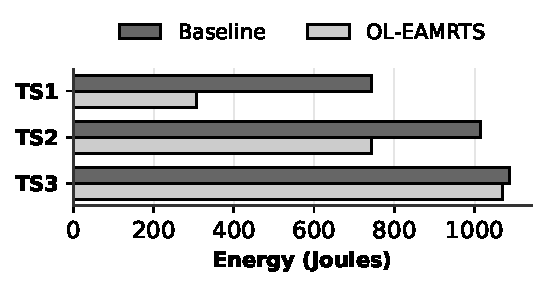
\includegraphics[width=0.65\columnwidth,keepaspectratio]{figures/energy_comparison.pdf}
    \caption{Energy consumption comparison across different task-sets.}
    \label{fig:energy_consumption}
\end{figure}

The overall system behavior is illustrated in Figure \ref{fig:system_behavior}, alongside Table \ref{tab:evaluation_migration}. Each 90-second evaluation window captures the stabilization of both migrations and \gls{dvfs} actuations. For task-set 1, the framework triggered a single migration at the \mbox{9-second} mark but revoked it two seconds later, stabilizing at the second-highest frequency. While previous ARM evaluations exhibited no migrations for this workload, this behavior is expected. On the ARM platforms, the task-set reached the maximum hardware frequency reduction (50\%) without needing to migrate. On RISC-V, after achieving a similar 50\% reduction, the heuristic attempted a migration to explore further down-scaling. Upon determining that a lower frequency was unsafe, the migration was correctly revoked.

Throughout this process, the \gls{ann} demonstrated high predictive accuracy. The first \gls{dvfs} actuation yielded utilization deviations of just 0.30\%, 2.34\%, and 0.02\% across cores 1, 2, and 3, respectively. The second actuation showed similarly low deviations of 2.04\%, 1.64\%, and 0.45\%. This precision allowed the framework to identify the second-highest frequency as the lowest safe operational level for task-set 1, successfully reaching the optimal energy configuration.

Finally, the RISC-V implementation achieved highly promising prediction accuracy compared to the baseline platforms. During the second actuation, the RISC-V average deviation of 1.38\% significantly outperformed the ARMv8 baseline (7.67\%) and closely approached the ARMv7 implementation (0.90\%).

The evaluation of task-set 2, which relied exclusively on online learning, further highlighted the hardware limitations of global \gls{pmu} counters. Because L2 cache events are tracked globally rather than per-core, memory-intensive operations on one core artificially inflate the counter readings for all concurrently executing tasks. Consequently, the framework erroneously interpreted purely CPU-bound workloads as contention-inducing and migrated them. Despite this, the system successfully revoked the incorrect migration and reached the lowest safe frequency within 34 seconds, achieving the optimal final energy configuration.

The \gls{ann}'s online adaptation proved capable of handling this volatility. Initial prediction deviations across cores 1, 2, and 3 were 6.13\%, 12.73\%, and 24.75\%. Following a migration, which degrades short-term accuracy by introducing novel task allocations, these deviations shifted to 37.96\%, 21.64\%, and 2.57\%. By the final \gls{dvfs} actuation, the \gls{ann} recovered to deviations of 12.53\%, 1.96\%, and 4.62\%. Compared to the ARMv7 baseline, which saw only moderate deviation increases (6.57\%, 7.93\%, and 12.20\%) after its first migration, the \mbox{RISC-V} implementation exhibited much steeper initial volatility. However, the continuous online learning successfully adapted the model and stabilized the system.

Lastly, for task-set 3, the migration heuristic successfully offloaded the image disparity task from the heavily oversubscribed core 3 to core 1, which hosted only a lightweight bandwidth task. While this migration effectively balanced the load and reduced core 3's utilization, the predicted utilizations at the next lower frequency consistently exceeded the safety margin. Thus, the framework correctly blocked any \gls{dvfs} downscaling, which would indeed lead to deadline misses.

\begin{figure}[ht]
    \centering
    
\includegraphics[width=0.9\columnwidth,keepaspectratio]{figures/shared_legend.pdf}
    \vspace{-2.5mm}
    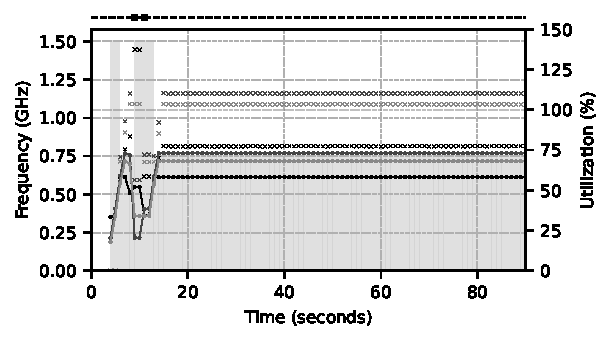
\includegraphics[width=\columnwidth,keepaspectratio]{figures/evaluation_taskset_1.pdf}
    \vspace{-2.5mm}
    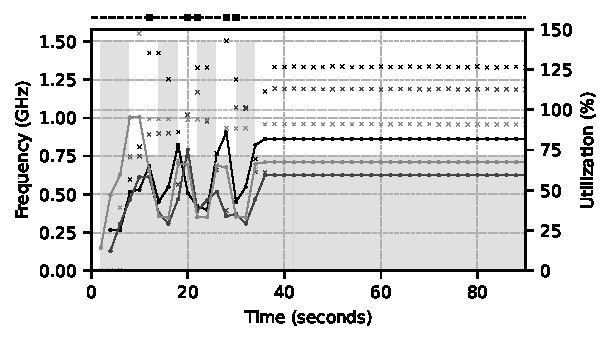
\includegraphics[width=\columnwidth,keepaspectratio]{figures/evaluation_taskset_2.pdf}
    \vspace{-3mm}
    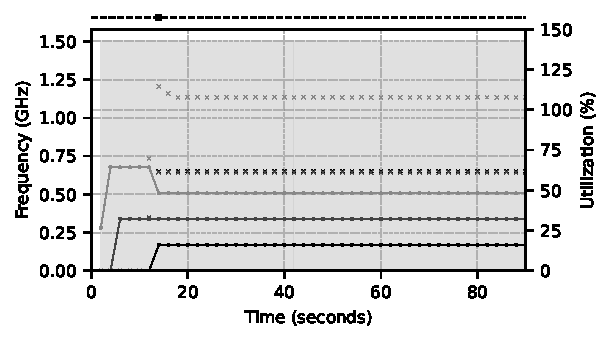
\includegraphics[width=\columnwidth,keepaspectratio]{figures/evaluation_taskset_3.pdf}
    \caption{System behavior over a 90-second evaluation window for task-set 1 (top), task-set 2 (middle), and task-set 3 (bottom).}
    \label{fig:system_behavior}
\end{figure}

\begin{table}[htb]
    \caption{Migrations for each task-set}
    \label{tab:evaluation_migration}
    \centering
    \begin{tabular}{|c|c|c|}
        \hline
        \textbf{Set} & \textbf{Time ($s$)} & \textbf{Description} \\ \hline
        \multirow{2}{*}{\textbf{TS1}}
                             & 9  & Migrate T4 (CPU-Hungry) from core 2 to core 1 \\
                             & 11 & Revoke last migration \\ \hline
        \multirow{5}{*}{\textbf{TS2}}
                             & 12 & Migrate T5 (CPU-Hungry) from core 3 to core 1 \\
                             & 20 & Migrate T5 (CPU-Hungry) from core 1 to core 2 \\
                             & 22 & Migrate T4 (CPU-Hungry) from core 2 to core 1 \\
                             & 28 & Migrate T5 (CPU-Hungry) from core 2 to core 1 \\
                             & 30 & Migrate T4 (CPU-Hungry) from core 1 to core 2 \\ \hline
        \multirow{1}{*}{\textbf{TS3}}
                             & 14 & Migrate T5 (Image disparity) from core 3 to core 1 \\ \hline
    \end{tabular}
\end{table}

\subsection{Runtime Overhead Analysis}

Over 2,107 iterations, the complete framework algorithm exhibited an average execution overhead of $102.75 \mu s$. Individually, the \gls{ann} prediction consumed $3.25 \mu s$, an incremental training pass averaged $3.71 \mu s$, and the migration heuristic required $10.5 \mu s$, compared to $1.81 \mu s$ and $5.13 \mu s$ for prediction and training in the original ARMv7 implementation. Integrating \gls{oleamrts} into the \gls{rtos} induced a negligible execution time increase of 0.46\% for memory-bound workloads and 0.16\% for hybrid workloads, against 0.18\% and 0.04\% in the original work. For purely CPU-bound tasks, no execution time increase was observed in either implementation.

\section{Discussion and Conclusion}

This evaluation successfully demonstrated the adaptability of \gls{oleamrts} to a fundamentally different micro-architecture. However, achieving this adaptation required changes to the profiling methodology. Specifically, the feature selection pipeline was modified to avoid selecting task-specific counters and those associated with idle noise.

While the framework consistently achieved the lowest safe \gls{dvfs} states across multiple workloads, operating on this new architecture also exposed hardware-specific limitations that temporarily disrupted prediction accuracy and induced unnecessary task migrations. Compared to previous ARM implementations, the \gls{ann} exhibited a steeper drop in prediction accuracy immediately following task migrations, indicating a difficulty in generalizing learned behaviors across new core allocations. Because the most critical contention indicators, L2 cache events, are strictly global on the target \gls{cots} platform, the framework cannot disambiguate between parallel CPU-bound and memory-bound workloads. Consequently, a purely CPU-bound task co-scheduled with a memory thrasher will inherit artificially high L2 contention readings, prompting the heuristic to erroneously migrate it in an attempt to alleviate shared resource contention.

% NOTE: This might not be the best way to frame the future contributions. But in my view it sounds reasonable.
Furthermore, while the coarse \gls{dvfs} granularity of the JH7110 \gls{soc} did not break the framework's operational safety, it restricted the fine-grained energy scaling observed in previous architectures. Ultimately, while this evaluation demonstrates that \gls{oleamrts} functions effectively on \mbox{RISC-V}, its performance can be significantly improved. Future work must investigate more advanced task behavior modeling techniques in order to overcome the limitations in hardware metrics and statistically select and derive useful metrics.

\bibliographystyle{IEEEtranN}
\small\bibliography{references}

\end{document}
